\section{Proposed architecture}

  Proposed predictor, as illustrated in figure~\ref{architecture}, takes ideas from both PConsC4~\cite{Michel383133} and 
  RaptorX-Contact~\cite{RaptorX} architectures (see section \ref{dlpredictors}).
  Global features, one-dimensional and two-dimensional features are being fed
  as input to the global, 1D and 2D modules, respectively.
  \begin{itemize}
    \item \textbf{Global module} is made of a succession of multiple fully-connected layers.
        Its output is repeated in order to match the dimensionality of the 1D module's input.
    \item \textbf{1D module} is a one-dimensional residual network.
        Each layer is composed of 1D convolution, 1D batch normalization and activation function.
        Its input is a concatenation of one-dimensional features and global module's output.
        A Kronecker product is applied between the module's output and itself
        in order to match the dimensionality of the 2D module's input.
    \item \textbf{2D module} is a two-dimensional residual network.
        Each layer is composed of 2D convolution, 2D batch normalization and activation function.
        Its input consists of a concatenation of the 2D features and the output of the 1D module.
  \end{itemize}
  The output of the 2D module is the output of the whole model. Contrary to RaptorX-Contact,
  it does not represent a single contact map but 5 contact maps predicted at contact thresholds
  $6$, $7.5$, $8$, $8.5$ and $10$ \AA{}, like in PConsC4.
  In contrast to the other two, proposed architecture is fully-convolutional and handles variable-length
  proteins even with a batch size greater than one.

  \begin{figure}[H]
    \begin{center}
      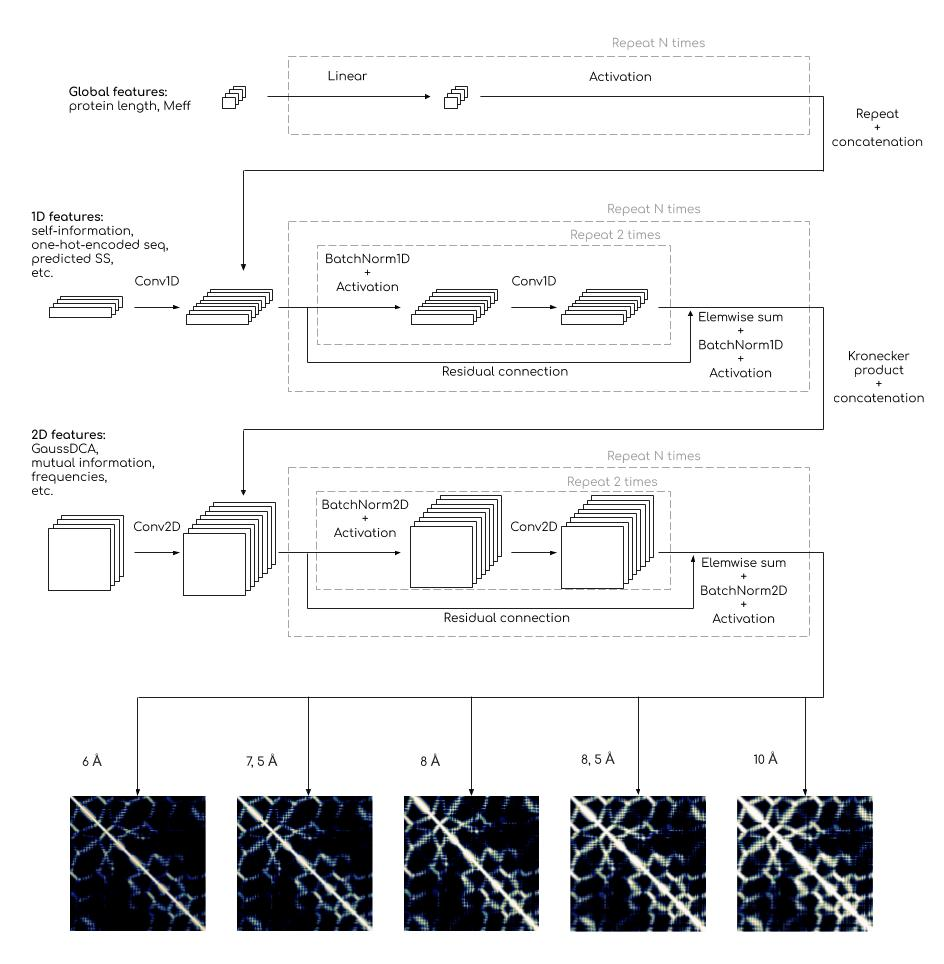
\includegraphics[width=\textwidth, keepaspectratio]{imgs/architecture.jpg}
       \caption{Proposed architecture of the deep convolutional neural network for semantic segmentation}
      \label{architecture}
    \end{center}
  \end{figure}